\part{Une structuration à reprendre : des tâches manuelles et semi-automatiques}

\clearpage
\thispagestyle{empty}
\cleardoublepage

\chapter{Outils, méthodologie et gestion du projet}


\section{Outils de développement}

\subsection{\gitlab}

La gestion quotidienne du programme \timeus{} se fait grâce à un dépôt sur \gitlab{}, un logiciel libre permettant aux entités comme Inria de créer une plate-forme interne de développement informatique. Sur \gitlab{} se trouve le dépôt central, organisé en plusieurs dossiers, dont un est réservé aux \odm. La technologie \textit{git} permet d'administrer les différentes versions du projet, sur une échelle à la fois verticale (les anciennes versions, appelées \commits, restant accessibles à travers un historique) et horizontale (le travail peut s'effectuer sur des \textit{branches} divergentes de la branche principale dite \master{} sans affecter l'état de cette dernière). Un commentaire est ajouté par l'utilisateur à chacun de ses \commits{} pour résumer ses modifications.

Chaque participant peut rapatrier le dépôt \gitlab{} en local pour travailler dessus ; ce rapatriement est un \textit{pull}. Il peut ensuite effectuer l'opération inverse, un \textit{push}, consistant à mettre ses \commits{} en ligne. Son équipe peut ainsi prendre connaissance des dernières avancées de la branche sur laquelle il travaille.

Une fois le travail dans une branche achevé, celle-ci peut être fusionnée avec \master. \gitlab{} propose une interface pour effectuer des \mergerequests{}. Il s'agit d'une demande de fusion, où \gitlab{} affiche l'historique de la branche. Les utilisateurs peuvent ainsi contrôler l'ensemble des \commits{} de la branche locale et vérifier qu'ils ne vont pas corrompre \master{} en créant des conflits (\textit{merge conflicts}).

\gitlab{} permet enfin à ses utilisateurs d'exposer un élément posant problème, d'effectuer des suggestions ou encore de porter à l'attention de leur équipe une ressource utile à travers des \issues{} (ou \textit{tickets}). Les \issues{} et les \mergerequests{} sont numérotées (\citecode{\#\textbackslash d} et \citecode{!\textbackslash d}\footnote{Par exemple, \citecode{\#5} fait référence à la cinquième \issue{} et \citecode{!5} à la cinquième \mergerequest{}.}), écrire leurs numéros dans \gitlab{} ou dans le commentaire de modification d'un \commit{} permettant de faire automatiquement référence à elles à travers un lien interne.

L'équipe ALMAnaCH possède un espace sur la plate-forme \gitlab{} d'Inria, où un dossier (en accès restreint) est réservé au programme \timeus{}. C'est ici, dans un sous-ensemble, que se trouve le dépôt des \odm. Le script \lse{} est déposé dans un dossier externe.

La branche \master{} compte quatre sous-dossiers :

\begin{itemize}
    \item \citecode{source} contient les treize fichiers XML-TEI des volumes des \odm{} ;
    \item \citecode{script} contient les scripts développés afin d'automatiser le traitement des fichiers ;
    \item \citecode{files} contient les fichiers XML-TEI générés à partir des fichiers sources et modifiés automatiquement ou à la main en vue de leur publication (monographies et fichiers de paratexte) ;
    \item \citecode{metadata} contient des fichiers de métadonnées sur le projet.
\end{itemize}

Ce dossier était notre espace de travail principal, notre première action ayant consisté en son rapatriement au niveau local. Notre méthodologie de travail était la suivante :

\begin{enumerate}
    \item Une branche était créée pour chaque mission ;
    \item Des \commits{} étaient effectués en local sur cette branche ;
    \item Les \commits{} d'une journée étaient mise en ligne sur \gitlab{} par un \textit{push} ;
    \item Lorsque la mission était achevée, une \mergerequest{} était ouverte ;
    \item La \mergerequest{} était acceptée et la branche fusionnée avec \master.
\end{enumerate}

\begin{figure}
    \centering
    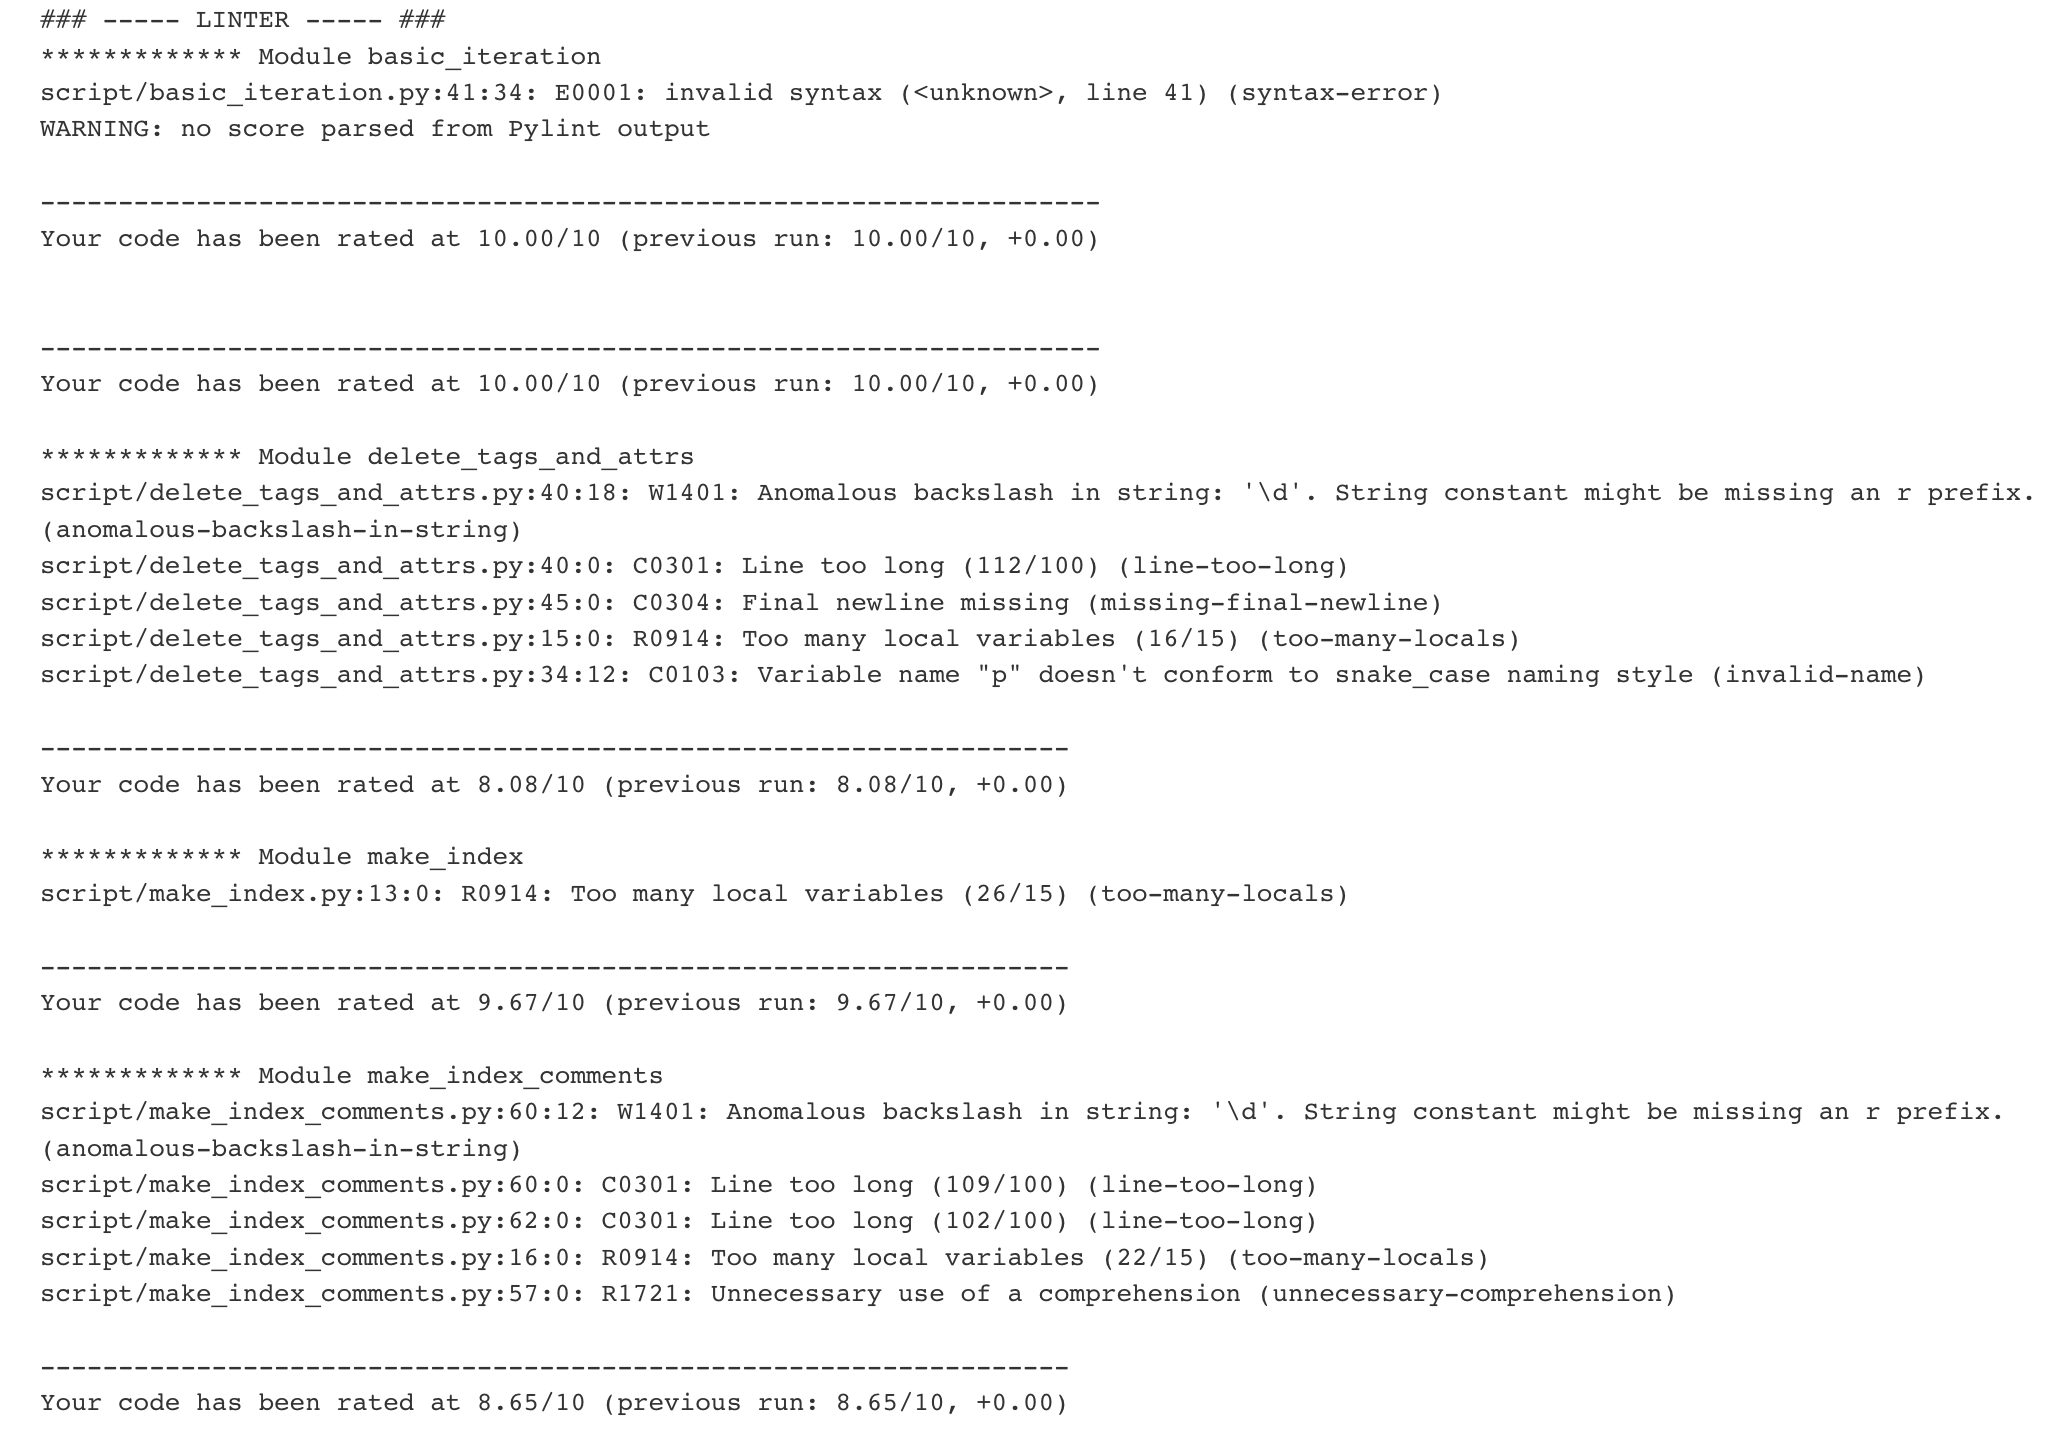
\includegraphics[width=15cm]{img/pylint_output.png}
    \caption{Exemple d'un contrôle de code par \textit{Pylint}, qui donne une note à chaque script (\textit{module}) et détaille ensuite les erreurs détectées.}
    \label{fig:pylint}
\end{figure}

Le \textit{linter} \textit{Pylint} était également implanté dans le dépôt ; il s'agit d'un système de vérification de code Python. Son rôle est de contrôler à chaque \textit{push} la qualité du code des scripts, notamment la longueur des lignes, les intitulés des variables ou encore la documentation des fonctions. Le résultat est affiché dans une console (\fig{} \ref{fig:pylint}).

\subsection{\pycharm{} et \oxygen}

Pour manipuler les fichiers XML, développer et activer les scripts Python, nous usions des logiciels \oxygen{} (éditeur de code XML sous licence propriétaire) et \pycharm{} (environnement de développement intégré pour la programmation en Python, une version est sous licence libre et une seconde sous licence propriétaire). 

Plusieurs fonctionnalités d'\oxygen{} ont facilité le traitement du corpus, notamment la possibilité de rassembler l'ensemble des fichiers dans un \og projet \fg. Par ce biais, des opérations --- par exemple effectuer une recherche ou remplacer une expression par une autre --- peuvent être menées sur le corpus sans requérir l'ouverture successive de chaque fichier. En outre, le logiciel dispose d'un système de vérification du code, qui là encore peut être appliqué à tout le corpus à travers l'outil \og projet \fg.

\pycharm{} est également équipé d'un outil de type \textit{linter} comparable à \textit{Pylint}, qui permet de s'assurer de la validité et de la lisibilité du code et facilite la programmation. \textit{Pylint} est cependant plus exigeant que le \textit{linter} natif de \pycharm, un double contrôle était donc nécessaire.

\section{Espaces de discussion}

La situation de confinement d'avril à mai et le maintien de la fermeture aux stagiaires des locaux d'Inria de juin à juillet a conduit à la mise en place d'outils de discussion.

\subsection{\Mattermost}

\Mattermost{} est un logiciel de discussion instantanée dont le code, écrit à l'origine sous un format propriétaire, a été publié en \opensource{}\footnote{Consultable sur \github{} (\url{https://github.com/mattermost/mattermost-server}, consulté le \today).} en 2015\footnote{Lindsay Brock, \textit{Open source Slack-alternative reaches 1.0: Self-host ready, Slack-compatible, MIT licensed}, 2 octobre 2015, \url{https://mattermost.com/blog/mattermost-3-4-16/} (consulté le \today).}. Auto-hébergé --- Inria stocke le code dans ses propres installations et n'a pas recours à un serveur distant ---, il s'agit de l'espace de discussion principal des agents d'Inria.

Composé de plusieurs \og chaînes \fg{} (\textit{public channels}) organisées de façon thématique, il leur permet d'échanger sur les différents projets et de suivre leur avancement, mais aussi d'exposer les difficultés techniques qu'ils rencontrent dans leur travail quotidien afin d'obtenir de l'aide. La chaîne \og \ocr \fg{} est ainsi fréquemment utilisée par les utilisateurs de \kraken{} (\fig{} \ref{fig:mattermost}).

\begin{figure}
    \centering
    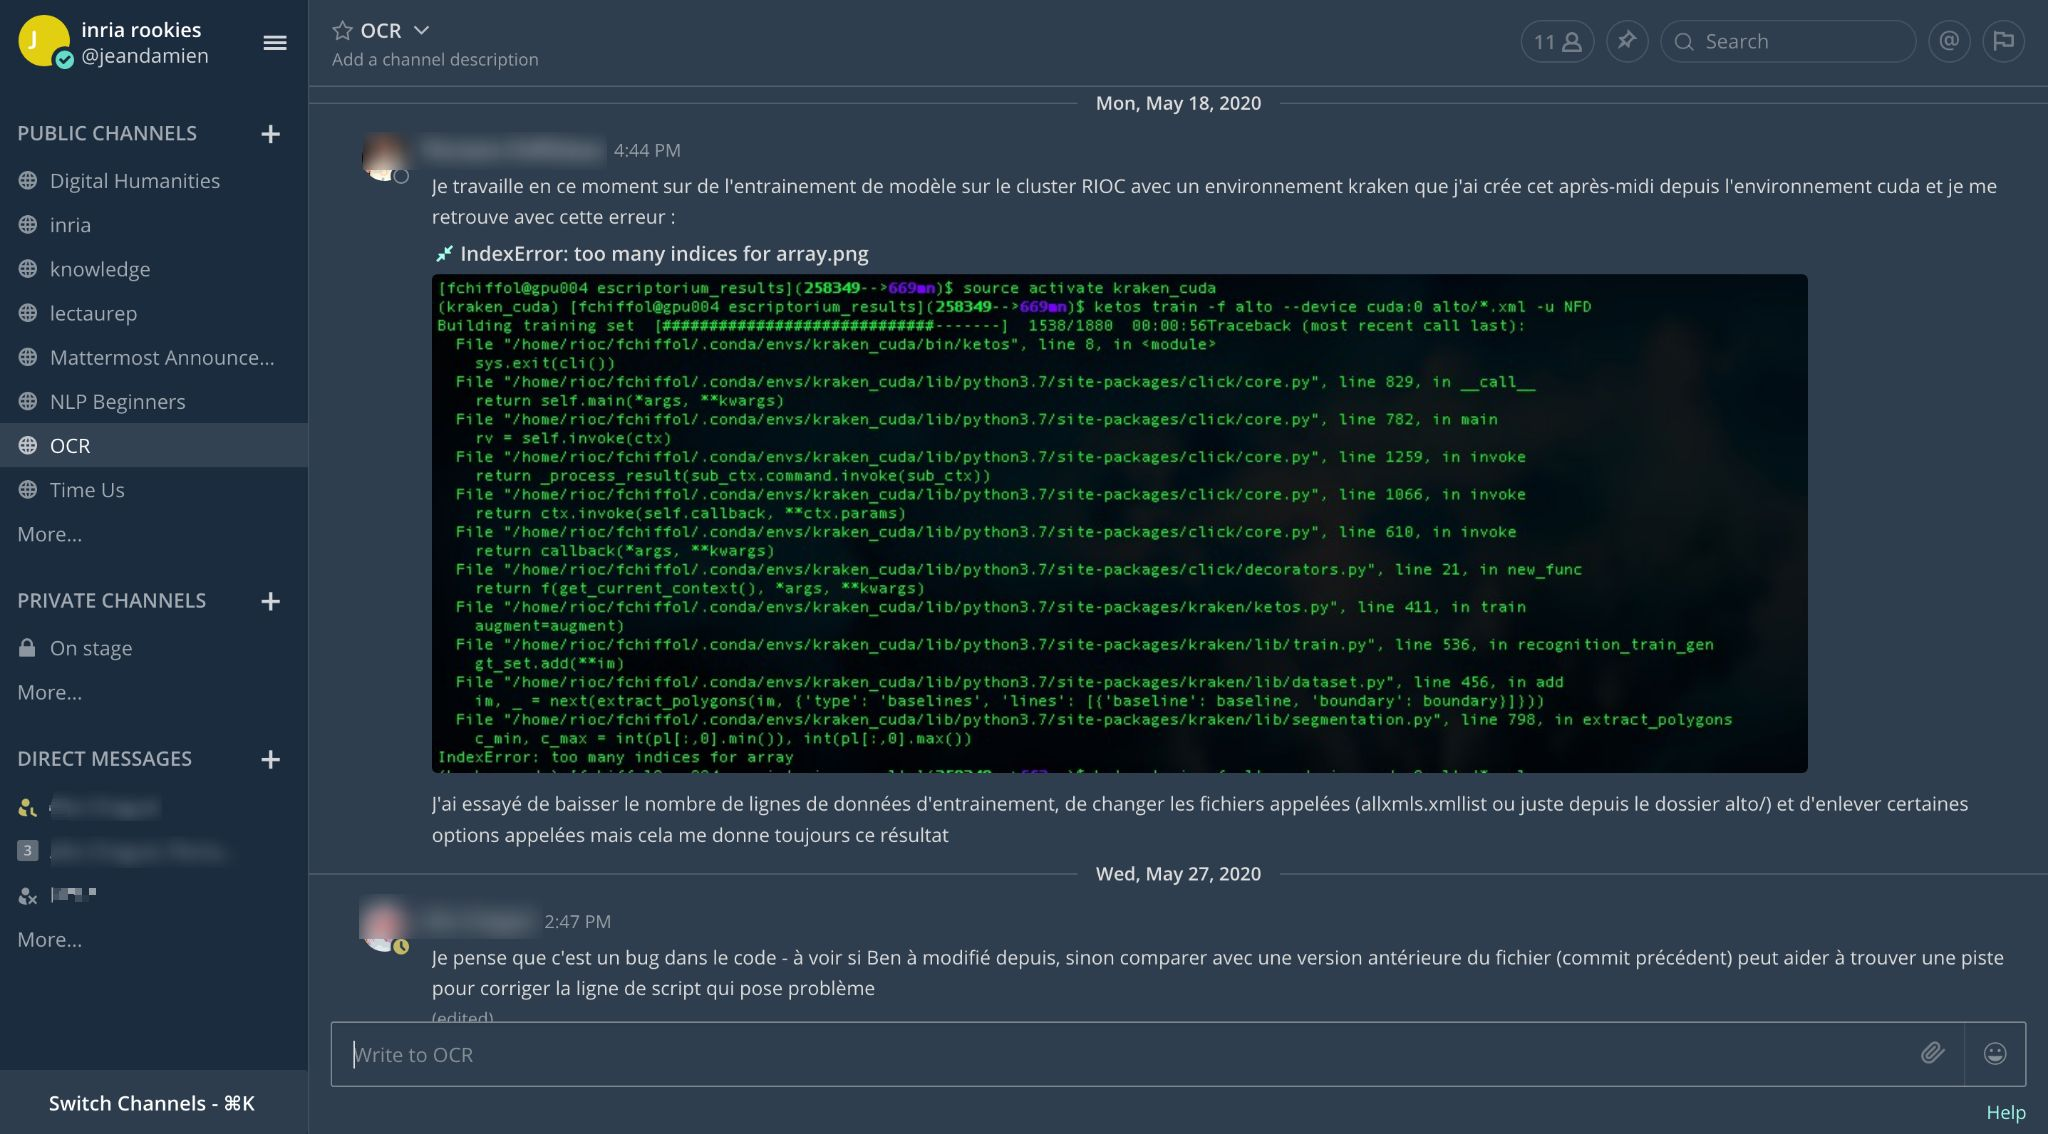
\includegraphics[width=16cm]{img/mattermost.jpg}
    \caption{Exemple de messages sur la chaîne \og \ocr \fg{} du \Mattermost{} d'Inria : une utilisatrice demande de l'aide au sujet d'une erreur dans l'exécution de \kraken{}. Sur le volet gauche se trouve la liste des chaînes disponibles.}
    \label{fig:mattermost}
\end{figure}

\subsection{\textit{Issues} et \mergerequests{} sur \gitlab}

Le programme \timeus{} possède également une chaîne ; cependant, pour les échanges afférents à nos missions, nous usions des espaces de discussion de \gitlab.

Les \issues{} et les \mergerequests{} n'ont en effet pas pour seule utilité de permettre aux utilisateurs d'exposer des problèmes ou de demander des fusions de branches. Il s'agit d'espaces dynamiques qui participent pleinement à la gestion de projet en offrant aux participants la possibilité de donner leur avis ou d'apporter des solutions, par exemple pour résoudre un \textit{merge conflict}.

Cet aspect est facilité par l'usage du langage à balises \markdown\footnote{\gitlab{} use de sa propre version du \markdown, le \textit{GitLab Flavored Markdown} : \url{https://docs.gitlab.com/ee/user/markdown.html} (consulté le \today).}. Il permet une mise en forme légère (listes, liens hypertexte, diagrammes), ainsi qu'une intégration d'échantillons de code. Si ceux-ci ne sont pas fonctionnels, le \markdown{} permet de leur appliquer une coloration syntaxique, les rendant ainsi plus facile à lire (\fig{} \ref{fig:ex_gitlab}).

Les échanges sur ces espaces restent accessibles après la clôture des \issues{} ou des \mergerequests{}, constituant ainsi un historique de l'avancement du projet.

\begin{figure}
    \centering
    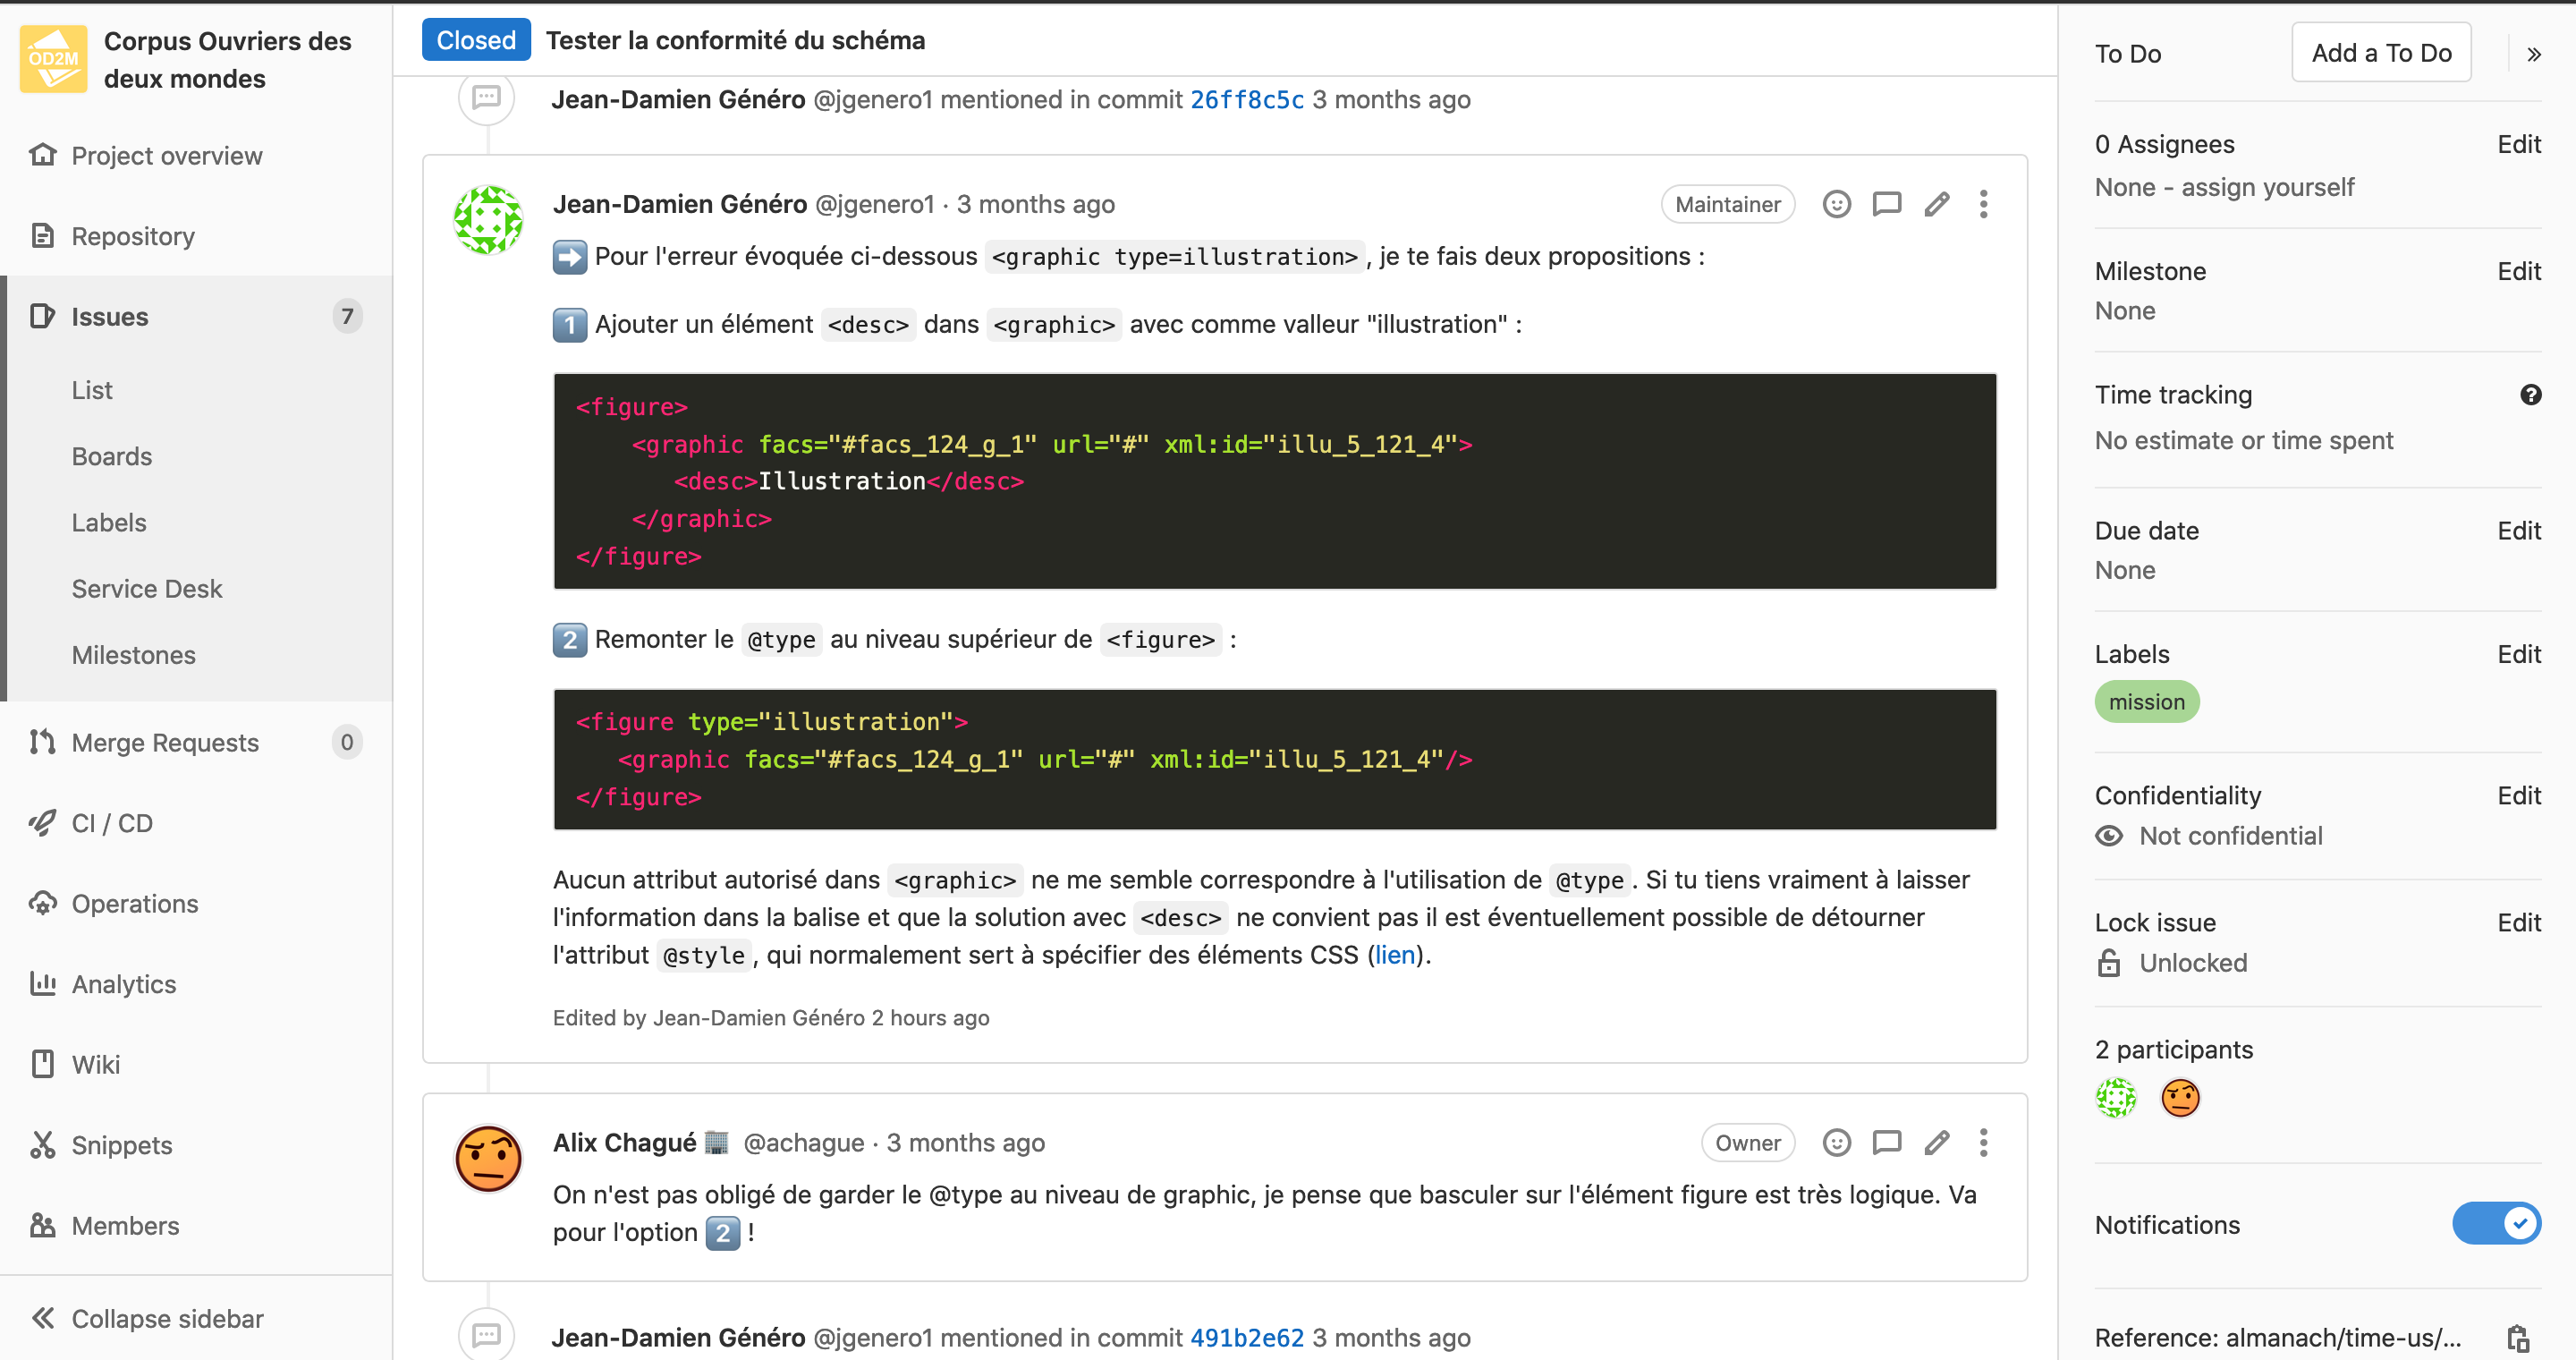
\includegraphics[width=16cm]{img/gitlab.png}
    \caption{Exemple de messages échangés avec une coloration syntaxique d'un code Python dans une \issue{} sur \gitlab.}
    \label{fig:ex_gitlab}
\end{figure}

\section{Feuille de route}

\subsection{Les missions du stage}

Au commencement de notre stage, huit \issues{} étaient ouvertes sur le \gitlab{} des \odm{}. Chacune correspondait à un problème ou à un point qui n'avait pas encore pu être développé. Elles constituaient donc notre \og feuille de route \fg, \cad{} l'exposé des missions que nous avions à réaliser (\ann{} \ref{ann:feuille_route}). Il nous a été demandé de les utiliser pour poser nos questions ou proposer nos solutions.

Les missions qui nous ont été confiées étaient de deux ordres.

Une première moitié consistait à contrôler les résultats du script \lse, tant au niveau du corpus qu'à celui de chaque fichier, et à effectuer des reprises si nécessaire. Tout d'abord, il s'agissait de détecter les erreurs de découpage des fichiers de volume et d'opérer les fusions ou les séparations nécessaires. Ceci avait pour but de donner à chaque fichier un identifiant unique après s'être assuré de l'unité de son contenu (\issue{}~1). Dans un second temps, nous devions nous intéresser à des éléments particuliers dans chaque fichier, à l'instar du contenu des balises \citecode{<facsimile>} (\issue{}~2), de la qualité des transcriptions (\issue{}~6) ou encore de la validité du schéma TEI (\issue{}~3); le contrôle de l'implémentation de la structure logique ayant constitué notre occupation principale.

L'autre moitié de nos missions avait pour but de valoriser les données des \odm{} en menant des actions ciblées. La principale consistait à identifier les individus enquêtés en liant les informations onomastiques du deuxième paragraphe (\textit{État civil de la famille}) à un tableau prosopographique établi par Stéphane Baciocchi, chercheur de l'EHESS (\issue{}~4). De plus, nous devions implémenter dans les fichiers un système permettant la citation de passages précis afin de faciliter les études des chercheurs du programme en leur offrant la possibilité d'établir un lien direct entre leur travail et les données contenues dans les fichiers XML (\issue{}~5).

Il nous a enfin été demandé de publier sur le blog Hypothèses de \timeus{} des billets rendant compte de notre travail\footnote{Consultable à cette adresse : \url{https://timeus.hypotheses.org/}.}.

\subsection{Une gestion de projet ?}

Nous n'avons pas utilisé d'outil véritablement dédié à la gestion de projet, détournant plutôt un outil courant de \gitlab, les \issues.

Des fonctionnalités de \gitlab{} sont pourtant dédiées à une gestion plus fine. La principale est l'outil \og tableau de bord \fg{} (\textit{boards}). Par défaut, les \issues{} sont affichées sous la forme d'une liste présentant toutes celles qui sont ouvertes, deux onglets permettant d'accéder à celles qui ont été résolues ou bien de les afficher toutes. Avec l'outil \og tableau de bord \fg{}, l'utilisateur a accès à un tableau de quatre colonnes, la première listant les issues ouvertes, la seconde affichant une liste de tâches (\textit{todo list}), la troisième présentant les tâches en cours (\textit{doing}) et la dernières les \issues{} terminées.

Au-delà de la présentation des tâches, le tableau de bord est également interactif. Ainsi, sélectionner une \issue{} affiche ses métadonnées (agent en charge de sa résolution, label, temps estimé, échéance). Un système de labels --- des étiquettes thématiques --- permet également de classer les \issues{} et les tâches de la \textit{todo list}. Le tableau de bord offre donc une vision globale du projet selon une organisation chronologique, tout en permettant des vues synthétiques ciblées.

Le fonctionnement des \textit{boards} de \gitlab{} est comparable à celui d'autres applications, comme par exemple \textit{Trello}. Il s'agit d'un organisateur de tâche, également sous forme de tableaux, qui est utilisé par ALMAnaCH et les Archives nationales pour coordonner le projet de lecture automatique des répertoires du Minutier central des notaires de Paris, Lectaurep.

Pour autant, ces outils ne sont utilisés ni dans le cadre général du programme \timeus, ni dans le cadre particulier des \odm. Plusieurs raisons peuvent l'expliquer. En premier lieu, \timeus{} s'appuie sur une documentation dont le caractère disparate --- tant géographique que chronologique et typologique --- se heurte à toute volonté de gestion centralisée, d'autant que chaque membre est chargé de la gestion de sa documentation locale.

Un tel outil doit également être constamment maintenu à jour afin de garantir un gain de productivité. À l'échelle des \odm{} et de notre stage, le nombre relativement faible de missions (8) et d'intervenants (2) ne justifiaient pas la mise en place du tableau de bord \gitlab{} ou la création d'un \textit{Trello}. L'affichage basique des \issues{} sous forme d'une liste se suffisait à lui-même.

\chapter{Contrôle du découpage des fichiers source}

\section{Les différents niveaux d'encodage}

L'encodage d'un texte brut s'effectue sur plusieurs niveaux, depuis une échelle documentaire surplombante jusqu'à celle plus fine de l'analyse scientifique. Ces niveaux sont décrits dans un document intitulé \textit{Best Practices for TEI in Libraries}, édité par le Consortium TEI et disponible en ligne\footcite[\textit{4.2. Encoding Levels}]{bestpratice}.

Le premier niveau est celui du découpage documentaire, soit la constitution d'un fichier qui reproduit le texte brut d'une unité codicologique et lui associe des métadonnées. Dans le cas des \odm, il s'agit du découpage des treize fichiers des volumes, qui ne s'est pas fait sans erreur.

Le second niveau est celui dit de l'encodage \og minimal \fg, dont le seul but est d'améliorer la navigation dans le document. Il s'agit d'identifier les paragraphes par des balises \citecode{<p>} et de liées celles-ci aux ensembles \citecode{<facsimile>} des images d'origine par un identifiant, tant en marquant les changements de page par des éléments \citecode{<pb>}.

Le troisième niveau s'intéresse au découpage éditorial, \cad{} à l'identification et à la reproduction de la structure logique du texte. Il s'agit d'un point crucial pour les fichiers des \odm, du fait de l'importance accordée par l'école leplaysienne à la structuration des monographies ; c'est également le niveau qui a nécessité la reprise la plus longue et la plus lourde.

Le quatrième niveau est celui de l'encodage sémantique, destiné à mettre en valeur les éléments internes au texte afin d'en faire une production électronique autonome. Dans les fichiers des \odm, cela s'est traduit par l'élimination des éléments de mise en page des volumes tels que les en-têtes ou les numéros de page.

Le cinquième et dernier niveau est celui de l'annotation scientifique. Pour l'équipe ALMAnaCH, il s'agissait de repérer les éléments d'onomastique et d'implanter un système permettant la citation de passage précis selon une granularité qui restait à définir.

L'ensemble de ces niveaux a été contrôlé lors du stage. Lorsqu'une correction était nécessaire, nous devions favoriser son automatisation par le biais de script Python. Cependant, ceci n’a pas toujours été possible, nous conduisant à engager des actions manuelles plus d'une fois.

\section{Vérification de la cohérence documentaire}

Nous avons commencé par contrôler le découpage des fichiers source, dont les résultats étaient étonnants pour certain volume. Ainsi, plus de trente fichiers avaient résulté du troisième volume de la deuxième série (\ann{} \ref{mappings2t3}). Au-delà d'une vérification de la cohérence du découpage, l'opération avait pour but, dans un premier temps, de reconnaître le contenu des fichiers et, dans un second temps, de lui associer un identifiant unique. La première 

\chapter[Correction des erreurs d'implémentation]{Correction des erreurs d'implémentation de la structure logique}

Début du chapitre 6.